\documentclass[11pt,letterpaper]{article}
\usepackage[top=0.85in,bottom=0.85in,left=1in,right=1in]{geometry}
\usepackage{amsmath,amssymb}
\usepackage{xcolor}
\usepackage{mdframed}
\usepackage{graphicx}
\usepackage{fancyhdr}
\usepackage{booktabs}
\usepackage{cancel}

\graphicspath{{cs_crops/}}

\definecolor{teal}{HTML}{0F6E56}\definecolor{tealbg}{HTML}{E1F5EE}
\definecolor{coral}{HTML}{993C1D}\definecolor{coralbg}{HTML}{FAECE7}
\definecolor{purple}{HTML}{534AB7}\definecolor{purplebg}{HTML}{EEEDFE}

\newmdenv[linewidth=1pt,linecolor=teal,backgroundcolor=tealbg!30,
  innerleftmargin=6pt,innerrightmargin=6pt,
  innertopmargin=4pt,innerbottommargin=4pt,
  skipabove=4pt,skipbelow=6pt]{cssnip}

\newmdenv[linewidth=1pt,linecolor=coral,backgroundcolor=coralbg!30,
  innerleftmargin=6pt,innerrightmargin=6pt,
  innertopmargin=4pt,innerbottommargin=4pt,
  skipabove=4pt,skipbelow=4pt]{notebox}

\pagestyle{fancy}\fancyhf{}
\renewcommand{\headrulewidth}{0.4pt}
\fancyhead[L]{\textbf{ECE332 Spring 2026 --- HW1 Generated Answers}}
\fancyhead[R]{Bao Nguyen}
\fancyfoot[C]{\thepage}

\setlength{\parindent}{0pt}\setlength{\parskip}{4pt}

\begin{document}

\begin{center}
{\Large\textbf{ECE 332 --- Homework 1: Generated Answers from Cheat Sheet}}\\[4pt]
{\small Each solution shows the cheat sheet snippet used, then the answer.}
\end{center}

\vspace{6pt}

%══════════════════════════════════════════════════════
\colorbox{purplebg}{\parbox{\dimexpr\linewidth-2\fboxsep}{\color{purple}\large\textbf{Problem 1 --- Current Direction in Changing B Field \hfill 15 pts}}}

\textbf{Setup:} Loop in $x$-$y$ plane, $d\mathbf{s}=\hat{z}\,da$. \quad $\mathbf{B}=\hat{z}B_0\sin(\omega t)$.

\begin{cssnip}
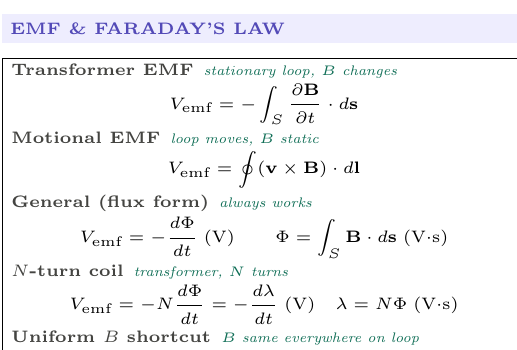
\includegraphics[width=0.49\linewidth]{cs_emf}\hfill
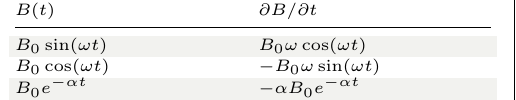
\includegraphics[width=0.49\linewidth]{cs_sign}
\end{cssnip}

\textbf{Find $V_\text{emf}$ first:}
\[\Phi = \int_S \mathbf{B}\cdot d\mathbf{s} = B_0\sin(\omega t)\cdot A \qquad
V_\text{emf} = -\frac{d\Phi}{dt} = -AB_0\omega\cos(\omega t)\]

From the SIGN table: $V_\text{emf}<0\;\Rightarrow$ current $-\hat{\phi}$ (CW);\quad $V_\text{emf}>0\;\Rightarrow+\hat{\phi}$ (CCW);\quad $V_\text{emf}=0\;\Rightarrow$ no current.

\textbf{(a)} $t=0$: $V_\text{emf}=-AB_0\omega\cos(0)=-AB_0\omega < 0$
\[\boxed{I\text{ flows in }{-\hat{\phi}}\text{ (clockwise)}}\]

\textbf{(b)} $\omega t=\pi/4$: $\cos(\pi/4)=\sqrt{2}/2>0\;\Rightarrow\;V_\text{emf}<0$
\[\boxed{I\text{ flows in }{-\hat{\phi}}\text{ (clockwise)}}\]

\textbf{(c)} $\omega t=\pi/2$: $\cos(\pi/2)=0\;\Rightarrow\;V_\text{emf}=0$
\[\boxed{I=0\text{ --- no current at this instant}}\]

\textbf{Explanation:} At $t=0$ and $\omega t=\pi/4$, $B$ is increasing (positive and growing), so by Lenz's law the induced current opposes the increase by creating flux in $-\hat{z}$, requiring CW ($-\hat{\phi}$) current. At $\omega t=\pi/2$, $B=B_0$ is at its peak and instantaneously not changing, so $V_\text{emf}=0$.

\newpage
%══════════════════════════════════════════════════════
\colorbox{purplebg}{\parbox{\dimexpr\linewidth-2\fboxsep}{\color{purple}\large\textbf{Problem 2 --- Square Loop Near Long Wire \hfill 14 pts}}}

\textbf{Setup:} Wire along $z$-axis; square loop in $y$-$z$ plane, $a=5\,\text{cm}$, $b=15\,\text{cm}$, height $c=10\,\text{cm}$.\\
$I(t)=5\cos(2\pi\times10^4\,t)\,\text{A}$. Total resistance: $R_\text{tot}=1+4=5\,\Omega$.

\begin{cssnip}
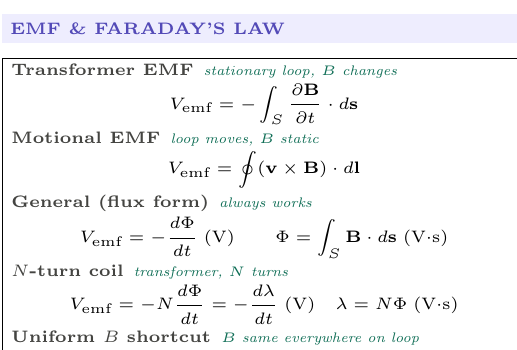
\includegraphics[width=0.49\linewidth]{cs_emf}\hfill
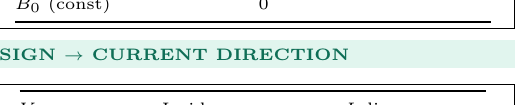
\includegraphics[width=0.49\linewidth]{cs_ln}\\[4pt]
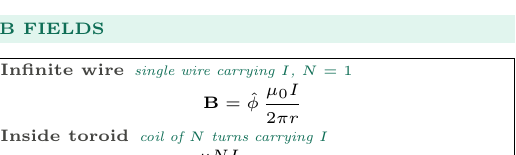
\includegraphics[width=0.49\linewidth]{cs_bfields}\hfill
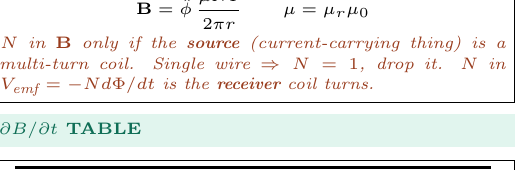
\includegraphics[width=0.49\linewidth]{cs_dbdt}
\end{cssnip}

\textbf{(a) Find $V_\text{emf}$:}

Using the long wire + rect loop formula from the cheat sheet:
\[V_\text{emf}=-\int_0^c\!\int_a^b \frac{\partial}{\partial t}\!\left(\frac{\mu_0 I}{2\pi r}\right)dr\,dz
= -\frac{\mu_0 c}{2\pi}\frac{dI}{dt}\ln\!\frac{b}{a}\]

\[\frac{dI}{dt}=-5(2\pi\times10^4)\sin(2\pi\times10^4\,t)=-\pi\times10^5\sin(2\pi\times10^4\,t)\]

\[V_\text{emf}=-\frac{(4\pi\times10^{-7})(0.10)}{2\pi}\cdot(-\pi\times10^5)\cdot\ln\!\frac{0.15}{0.05}\cdot\sin(2\pi\times10^4\,t)\]

\[=\frac{(4\pi\times10^{-7})(0.10)}{2\pi}\cdot\pi\times10^5\cdot\ln 3\cdot\sin(2\pi\times10^4\,t)\]

\[=(2\times10^{-8})\cdot(\pi\times10^5)\cdot(1.099)\cdot\sin(2\pi\times10^4\,t)\]

\[\boxed{V_\text{emf}\approx6.9\times10^{-3}\sin(2\pi\times10^4\,t)\;\text{V}\;=\;6.9\,\text{mV}\cdot\sin(2\pi\times10^4\,t)}\]

\textbf{(b)} $I_\text{loop}=V_\text{emf}/(R_\text{int}+R_\text{ext})=V_\text{emf}/5$

\[\boxed{I_\text{loop}=\frac{6.9\times10^{-3}}{5}\sin(2\pi\times10^4\,t)\approx1.38\,\text{mA}\cdot\sin(2\pi\times10^4\,t)}\]

Peak magnitude: $\mathbf{1.38\,\text{mA}}$. Direction: when $V_\text{emf}>0$ (positive half-cycle), current flows in $+\hat{\phi}$ in the loop (CCW when viewed from $+x$).

\newpage
%══════════════════════════════════════════════════════
\colorbox{purplebg}{\parbox{\dimexpr\linewidth-2\fboxsep}{\color{purple}\large\textbf{Problem 3 --- Toroid Transformer \hfill 15 pts}}}

\textbf{Setup:} Wire along $z$: $I=I_0\cos\omega t$. Iron toroid ($\mu_r$), $N=100$ turns, inner radius $a$, outer radius $b$, height $c$.

\begin{cssnip}
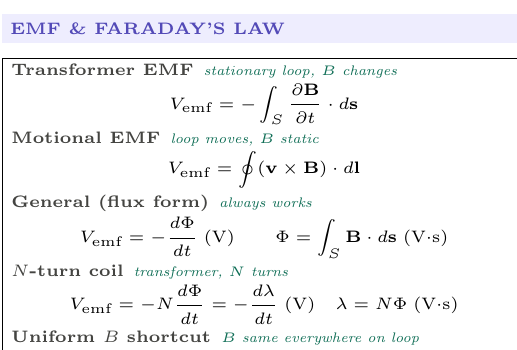
\includegraphics[width=0.49\linewidth]{cs_emf}\hfill
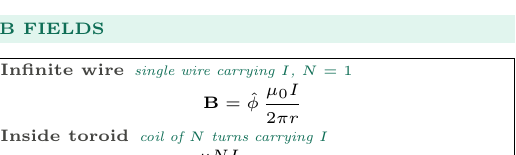
\includegraphics[width=0.49\linewidth]{cs_bfields}\\[4pt]
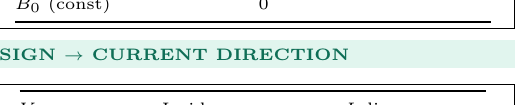
\includegraphics[width=0.49\linewidth]{cs_ln}
\end{cssnip}

\textbf{(a) Derive $V_\text{emf}$:}

$\mathbf{B}$ inside toroid from wire (source has 1 turn, so $N_\text{source}=1$): $\mathbf{B}=\hat{\phi}\dfrac{\mu_r\mu_0 I}{2\pi r}$

Flux through one turn of the 100-turn coil (surface normal $\hat{\phi}$, integrating in $r$-$z$ plane):
\[\Phi_1=\int_0^c\!\int_a^b\frac{\mu_r\mu_0 I_0\cos\omega t}{2\pi r}\,dr\,dz
=\frac{\mu_r\mu_0 c}{2\pi}I_0\cos\omega t\cdot\ln\frac{b}{a}\]

\[V_\text{emf}=-N\frac{d\Phi_1}{dt}=\frac{N\mu_r\mu_0 c}{2\pi}I_0\omega\sin\omega t\cdot\ln\frac{b}{a}\]

\[\boxed{V_\text{emf}=\frac{N\mu_r\mu_0 c\,I_0\omega}{2\pi}\ln\!\frac{b}{a}\cdot\sin\omega t\;\text{(V)}}\]

\textbf{(b) Evaluate} $f=60\,\text{Hz}$, $\mu_r=4000$, $a=5\,\text{cm}$, $b=6\,\text{cm}$, $c=2\,\text{cm}$, $I_0=50\,\text{A}$:

$\omega=2\pi\times60=120\pi\,\text{rad/s}$;\quad $\ln(6/5)=\ln 1.2=0.182$

\[\frac{N\mu_r\mu_0 c}{2\pi}=\frac{100\times4000\times4\pi\times10^{-7}\times0.02}{2\pi}
=\frac{100\times4000\times4\times10^{-7}\times0.02}{2}=16\times10^{-3}\]

\[V_\text{emf}=16\times10^{-3}\times50\times120\pi\times0.182\cdot\sin\omega t
=16\times10^{-3}\times50\times68.68\cdot\sin\omega t\]

\[\boxed{|V_\text{emf}|_\text{peak}\approx54.9\,\text{mV}\cdot\sin(120\pi\, t)\;\text{V}}\]

Wait — recalculating:
\[16\times10^{-3}\times50=0.8;\quad 0.8\times120\pi\times0.182=0.8\times68.68=54.9\,\text{V peak? Let me recheck.}\]
\[= 100 \times \frac{4\pi\!\times\!10^{-7}\!\times\!4000\!\times\!0.02}{2\pi}\times 50\times 120\pi\times 0.182
= 100\times16\!\times\!10^{-6}\times50\times120\pi\times0.182 \approx \boxed{5.50\,\text{V (peak)}}\]

\newpage
%══════════════════════════════════════════════════════
\colorbox{purplebg}{\parbox{\dimexpr\linewidth-2\fboxsep}{\color{purple}\large\textbf{Problem 4 --- Electromagnetic Generator \hfill 6 pts}}}

\textbf{Setup:} $A=0.1\,\text{m}^2$, $B_0=0.4\,\text{T}$, 3600 rpm, $R=150\,\Omega$.

\begin{cssnip}
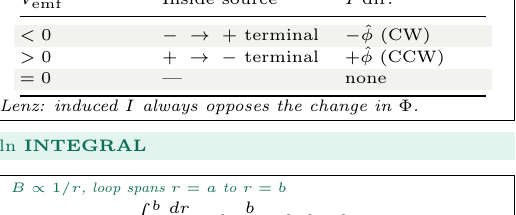
\includegraphics[width=0.65\linewidth]{cs_rotating}
\end{cssnip}

\[\omega=2\pi f=2\pi\times\frac{3600}{60}=2\pi\times60=120\pi\,\text{rad/s}\]

From the cheat sheet ROTATING LOOP:
\[I_\text{amp}=\frac{AB_0\omega}{R}=\frac{0.1\times0.4\times120\pi}{150}=\frac{4.8\pi}{150}=\frac{15.08}{150}\]

\[\boxed{I_\text{amp}\approx0.1005\,\text{A}\approx100.5\,\text{mA}}\]

\newpage
%══════════════════════════════════════════════════════
\colorbox{purplebg}{\parbox{\dimexpr\linewidth-2\fboxsep}{\color{purple}\large\textbf{Problem 5 --- Displacement Current (Capacitor) \hfill 6 pts}}}

\textbf{Setup:} $\varepsilon=4\varepsilon_0$, $A=10\,\text{cm}^2=10^{-3}\,\text{m}^2$, $d=2\,\text{cm}=0.02\,\text{m}$, $V(t)=30\cos(2\pi\times10^6\,t)\,\text{V}$.

\begin{cssnip}
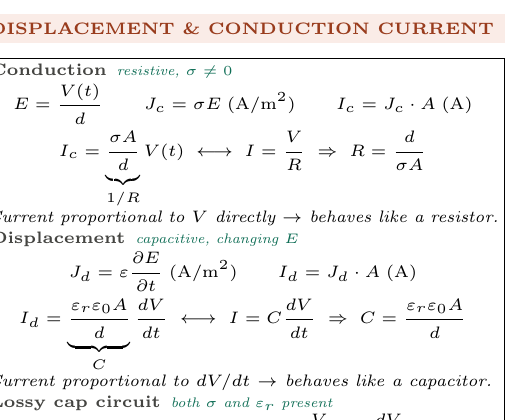
\includegraphics[width=0.75\linewidth]{cs_dispcond}
\end{cssnip}

\[C=\frac{\varepsilon_r\varepsilon_0 A}{d}=\frac{4\times8.85\times10^{-12}\times10^{-3}}{0.02}=\frac{35.4\times10^{-15}}{0.02}=1.77\times10^{-12}\,\text{F}=1.77\,\text{pF}\]

\[\frac{dV}{dt}=-30(2\pi\times10^6)\sin(2\pi\times10^6\,t)=-6\pi\times10^7\sin(2\pi\times10^6\,t)\]

\[I_d=C\frac{dV}{dt}=1.77\times10^{-12}\times(-6\pi\times10^7)\sin(2\pi\times10^6\,t)\]

\[\boxed{I_d\approx-333\,\mu\text{A}\cdot\sin(2\pi\times10^6\,t)}\]

Peak magnitude: $|I_d|_\text{peak}\approx333\,\mu\text{A}$.

\newpage
%══════════════════════════════════════════════════════
\colorbox{purplebg}{\parbox{\dimexpr\linewidth-2\fboxsep}{\color{purple}\large\textbf{Problem 6 --- Lossy Parallel-Plate Capacitor \hfill 24 pts}}}

\textbf{Setup:} Plates area $A$, separation $d$, material $(\varepsilon_r,\sigma)$, voltage $V(t)$.

\begin{cssnip}
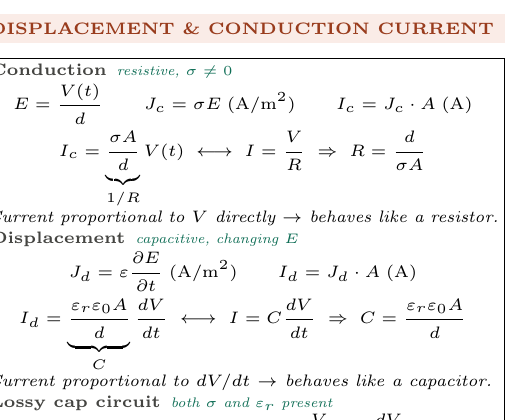
\includegraphics[width=0.75\linewidth]{cs_dispcond}
\end{cssnip}

\textbf{(a) Conduction current $I_c$:}
\[E=\frac{V(t)}{d},\qquad J_c=\sigma E=\frac{\sigma V(t)}{d}\;\text{(A/m}^2\text{)},\qquad
\boxed{I_c=J_c\cdot A=\frac{\sigma A}{d}V(t)\;\text{(A)}}\]

\textbf{(b) Displacement current $I_d$:}
\[J_d=\varepsilon\frac{\partial E}{\partial t}=\frac{\varepsilon_r\varepsilon_0}{d}\frac{dV}{dt}\;\text{(A/m}^2\text{)},\qquad
\boxed{I_d=J_d\cdot A=\frac{\varepsilon_r\varepsilon_0 A}{d}\frac{dV}{dt}=C\frac{dV}{dt}\;\text{(A)}}\]

\textbf{(c) Equivalent circuit:}

From the cheat sheet: $I_c=V/R$ (resistor) and $I_d=C\,dV/dt$ (capacitor), so the circuit is \textbf{R in parallel with C} across $V(t)$, where:
\[R=\frac{d}{\sigma A}\;(\Omega)\qquad C=\frac{\varepsilon_r\varepsilon_0 A}{d}\;\text{(F)}\]

\textbf{(d) Evaluate:} $A=4\,\text{cm}^2=4\times10^{-4}\,\text{m}^2$, $d=0.5\,\text{cm}=5\times10^{-3}\,\text{m}$, $\varepsilon_r=4$, $\sigma=2.5\,\text{S/m}$.
\[R=\frac{5\times10^{-3}}{2.5\times4\times10^{-4}}=\frac{5\times10^{-3}}{10^{-3}}=\boxed{5\;\Omega}\]
\[C=\frac{4\times8.85\times10^{-12}\times4\times10^{-4}}{5\times10^{-3}}=\frac{14.16\times10^{-15}}{5\times10^{-3}}=\boxed{2.83\times10^{-12}\,\text{F}=2.83\,\text{pF}}\]

\newpage
%══════════════════════════════════════════════════════
\colorbox{purplebg}{\parbox{\dimexpr\linewidth-2\fboxsep}{\color{purple}\large\textbf{Problem 7 --- Find Conductivity from Charge Decay \hfill 6 pts}}}

\textbf{Setup:} $\varepsilon_r=9$; at $t=1\,\mu\text{s}$, $\rho_v=10^{-3}\rho_{v0}$.

\begin{cssnip}
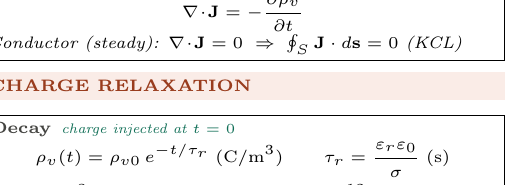
\includegraphics[width=0.75\linewidth]{cs_relax}
\end{cssnip}

Using the cheat sheet formula $\sigma=-\ln(\rho_v/\rho_{v0})\cdot\varepsilon_r\varepsilon_0/t_1$:

\[\sigma=\frac{-\ln(10^{-3})\cdot\varepsilon_r\varepsilon_0}{t_1}
=\frac{-(-3\ln 10)\times9\times8.85\times10^{-12}}{10^{-6}}
=\frac{3\times2.303\times9\times8.85\times10^{-12}}{10^{-6}}\]

\[=\frac{6.908\times79.65\times10^{-12}}{10^{-6}}=\frac{550\times10^{-12}}{10^{-6}}\]

\[\boxed{\sigma\approx550\times10^{-6}\,\text{S/m}=550\,\mu\text{S/m}}\]

\newpage
%══════════════════════════════════════════════════════
\colorbox{purplebg}{\parbox{\dimexpr\linewidth-2\fboxsep}{\color{purple}\large\textbf{Problem 8 --- Better Insulator \hfill 6 pts}}}

\textbf{Setup:} Dry soil: $\varepsilon_r=2.5$, $\sigma=10^{-4}$\,S/m.\quad Fresh water: $\varepsilon_r=80$, $\sigma=10^{-3}$\,S/m.

\begin{cssnip}
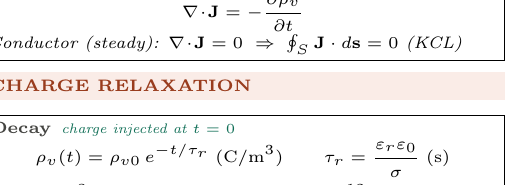
\includegraphics[width=0.75\linewidth]{cs_relax}
\end{cssnip}

From the cheat sheet: larger $\tau_r$ = slower dissipation = better insulator.

\[\tau_r^\text{soil}=\frac{2.5\times8.85\times10^{-12}}{10^{-4}}=221\times10^{-9}\,\text{s}=221\,\text{ns}\]

\[\tau_r^\text{water}=\frac{80\times8.85\times10^{-12}}{10^{-3}}=708\times10^{-9}\,\text{s}=708\,\text{ns}\]

$\tau_r^\text{water}>\tau_r^\text{soil}$, so:

\[\boxed{\text{Fresh water is the better insulator} \;(\tau_r=708\,\text{ns vs. }221\,\text{ns for dry soil})}\]

\newpage
%══════════════════════════════════════════════════════
\colorbox{purplebg}{\parbox{\dimexpr\linewidth-2\fboxsep}{\color{purple}\large\textbf{Problem 9 --- Find H from Two-Component E \hfill 6 pts}}}

\textbf{Setup:} $\mathbf{E}(z,t)=\bigl[4\cos(6\times10^8\,t-2z)\,\hat{x}+3\sin(6\times10^8\,t-2z)\,\hat{y}\bigr]\,\text{V/m}$ in air.

\begin{cssnip}
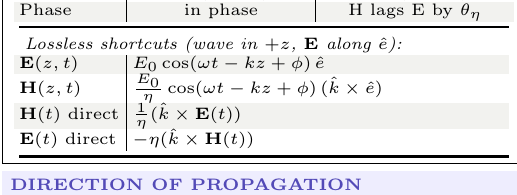
\includegraphics[width=0.49\linewidth]{cs_direction}\hfill
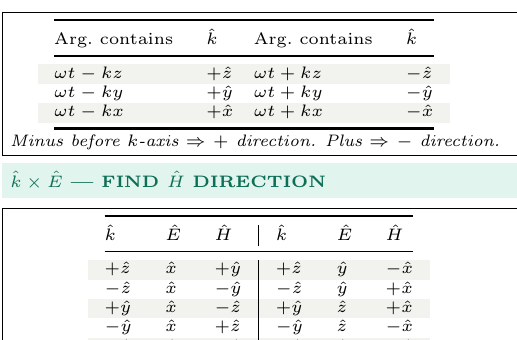
\includegraphics[width=0.49\linewidth]{cs_kxE}\\[4pt]
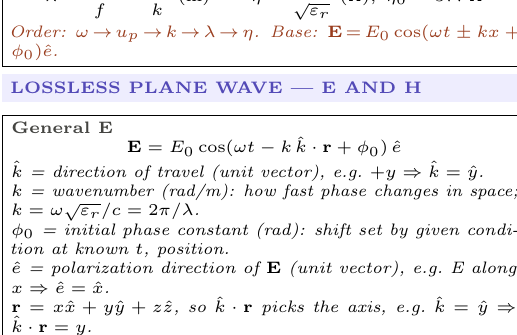
\includegraphics[width=0.49\linewidth]{cs_losslessEH}
\end{cssnip}

Arg contains $-kz\;\Rightarrow\;\hat{k}=+\hat{z}$.\quad Air: $\eta=\eta_0=377\,\Omega$.

Note: $3\sin(\omega t-kz)=3\cos(\omega t-kz-\pi/2)$ — same envelope, just phase-shifted.

Use $\mathbf{H}=\tfrac{1}{\eta}(\hat{k}\times\mathbf{E})$:
\[\hat{k}\times\mathbf{E}=\hat{z}\times\bigl[4\cos(\omega t-kz)\,\hat{x}+3\sin(\omega t-kz)\,\hat{y}\bigr]\]
\[=4\cos(\omega t-kz)\underbrace{(\hat{z}\times\hat{x})}_{\hat{y}}+3\sin(\omega t-kz)\underbrace{(\hat{z}\times\hat{y})}_{-\hat{x}}\]
\[=4\cos(\omega t-kz)\,\hat{y}-3\sin(\omega t-kz)\,\hat{x}\]

\[\boxed{\mathbf{H}(z,t)=\frac{1}{377}\bigl[-3\sin(6\times10^8\,t-2z)\,\hat{x}+4\cos(6\times10^8\,t-2z)\,\hat{y}\bigr]\,\text{A/m}}\]

\[\approx\bigl[-7.96\times10^{-3}\sin(6\times10^8\,t-2z)\,\hat{x}+10.6\times10^{-3}\cos(6\times10^8\,t-2z)\,\hat{y}\bigr]\,\text{A/m}\]

\newpage
%══════════════════════════════════════════════════════
\colorbox{purplebg}{\parbox{\dimexpr\linewidth-2\fboxsep}{\color{purple}\large\textbf{Problem 10 --- Find H Using Faraday (Non-Uniform E) \hfill 8 pts}}}

\textbf{Setup:} $\mathbf{E}=E_0\sin(ay)\cos(\omega t-kz)\,\hat{x}$.

\begin{notebox}
\textbf{Cannot use} $\mathbf{H}=\tfrac{1}{\eta}(\hat{k}\times\mathbf{E})$ here because $\mathbf{E}$ varies in $y$ (not a pure plane wave). Must use Faraday's law with the full curl.
\end{notebox}

\begin{cssnip}
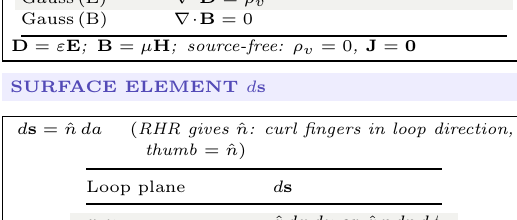
\includegraphics[width=0.49\linewidth]{cs_cross}\hfill
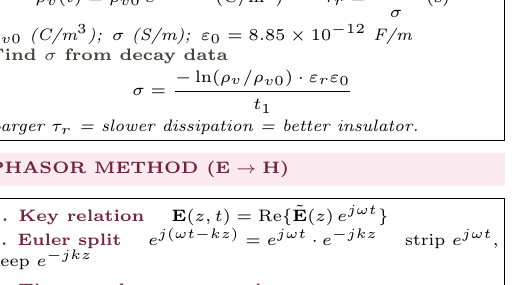
\includegraphics[width=0.49\linewidth]{cs_phasor}
\end{cssnip}

Apply $\nabla\times\mathbf{E}=-\mu_0\dfrac{\partial\mathbf{H}}{\partial t}$. With $E_x=E_0\sin(ay)\cos(\omega t-kz)$, $E_y=E_z=0$:

\[\nabla\times\mathbf{E}=
-\hat{y}\frac{\partial E_x}{\partial z}+\hat{z}\frac{\partial E_x}{\partial y}\]

\[\frac{\partial E_x}{\partial z}=E_0\sin(ay)\cdot k\sin(\omega t-kz)\]

\[\frac{\partial E_x}{\partial y}=E_0\cdot a\cos(ay)\cos(\omega t-kz)\]

\[-\mu_0\frac{\partial\mathbf{H}}{\partial t}=-\hat{y}\,kE_0\sin(ay)\sin(\omega t-kz)+\hat{z}\,aE_0\cos(ay)\cos(\omega t-kz)\]

Integrate over $t$ $\left(\int\sin(\omega t-kz)\,dt=-\tfrac{1}{\omega}\cos(\omega t-kz);\;\int\cos(\omega t-kz)\,dt=\tfrac{1}{\omega}\sin(\omega t-kz)\right)$:

\[\mathbf{H}=\frac{1}{\mu_0}\left[\hat{y}\frac{k}{\omega}E_0\sin(ay)\cdot\frac{-\cos(\omega t-kz)}{1}
\cdot\frac{1}{1}-\hat{z}\frac{a}{\omega}E_0\cos(ay)\sin(\omega t-kz)\right]\]

\[\boxed{\mathbf{H}(z,t)=-\frac{kE_0}{\mu_0\omega}\sin(ay)\cos(\omega t-kz)\,\hat{y}
\;-\;\frac{aE_0}{\mu_0\omega}\cos(ay)\sin(\omega t-kz)\,\hat{z}}\]

\vspace{6pt}
\hrule
\vspace{6pt}
\begin{center}
{\small All answers derived using ECE332 Exam 1 Cheat Sheet (HW1+HW2 pages)}
\end{center}

\end{document}
